\documentclass[10pt]{beamer}

\usetheme[progressbar=frametitle]{metropolis}
\usepackage{appendixnumberbeamer}

\usepackage{booktabs}
\usepackage{ulem}

\usepackage[scale=2]{ccicons}
\usepackage{pgfplots}
\usepgfplotslibrary{dateplot}
\usepackage{xspace}
\newcommand{\themename}{\textbf{\textsc{metropolis}}\xspace}
\usepackage[justification=centering]{caption}
\captionsetup{labelformat=empty,labelsep=none}
\usepackage{enumerate}   
\setbeamertemplate{section in toc}[sections numbered]

\title{Formation Git}
\date{11/05/2023}
\author{Nicolas Barrier \and Witold Podlejski \and Criscely
Lujan-Paredes}
\date{}

\makeatletter
\setlength{\metropolis@titleseparator@linewidth}{2pt}
\setlength{\metropolis@progressonsectionpage@linewidth}{2pt}
\setlength{\metropolis@progressinheadfoot@linewidth}{2pt}
\makeatother

\definecolor{RRR}{rgb}{0.702,0.2,0.2}
\definecolor{bleuclair}{rgb}{0.9,0.9,1}
\definecolor{grisbleu}{rgb}{0.85,0.85,1}
\definecolor{monbleu}{rgb}{0,0.4,0.6}
\definecolor{bleuclair}{rgb}{0.9,0.9,1}
\definecolor{autrebleu}{rgb}{0.15,0.5,0.65}
\definecolor{bleufond}{rgb}{0.59,0.66,0.81}
\definecolor{bleufondplus}{rgb}{0.21,0.29,0.47}
\definecolor{monrouge}{rgb}{1,0.16,0.14}
\definecolor{denim}{rgb}{0.08, 0.38, 0.74}
 \definecolor{cornflowerblue}{rgb}{0.39, 0.58, 0.93}

\definecolor{flame}{rgb}{0.89, 0.35, 0.13}
\hypersetup{colorlinks,linkcolor=,urlcolor=cornflowerblue}
\newcommand{\code}[1]{\textit{\ttfamily\textcolor{flame}{#1}}}


%\setbeamercolor{normal text}{bg=white}
%\setbeamercolor{alerted text}{fg=red}
% \setbeamercolor{example text}{fg=green!50!black}
% \setbeamercolor{structure}{fg=beamer@blendedblue}
\setbeamercolor{background canvas}{bg=white}
% \setbeamercolor{background}{bg=green, fg=red}
% \setbeamercolor{palette primary}{use=structure,fg=structure.fg}
% \setbeamercolor{palette secondary}{use=structure,fg=structure.fg!75!black}
% \setbeamercolor{palette tertiary}{use=structure,fg=structure.fg!50!black}
% \setbeamercolor{palette quaternary}{fg=black}
% \setbeamercolor{palette sidebar primary}{use=normal text,fg=normal text.fg}
% \setbeamercolor{palette sidebar secondary}{use=structure,fg=structure.fg}
% \setbeamercolor{palette sidebar tertiary}{use=normal text,fg=normal text.fg}
% \setbeamercolor{palette sidebar quaternary}{use=structure,fg=structure.fg}
% \setbeamercolor{math text}{}
% \setbeamercolor{math text inlined}{parent=math text}
% \setbeamercolor{math text displayed}{parent=math text}
% \setbeamercolor{normal text in math text}{}
% \setbeamercolor{local structure}{parent=structure}
% \setbeamercolor{titlelike}{parent=structure}
% \setbeamercolor{title}{parent=titlelike}
% \setbeamercolor{title in head/foot}{parent=palette quaternary}
% \setbeamercolor{title in sidebar}{parent=palette sidebar quaternary}
% \setbeamercolor{subtitle}{parent=title}
% \setbeamercolor{author}{}
% \setbeamercolor{author in head/foot}{parent=palette primary}
% \setbeamercolor{author in sidebar}{use=palette sidebar tertiary,fg=palette sidebar tertiary.fg}
% \setbeamercolor{institute}{}
% \setbeamercolor{institute in head/foot}{parent=palette tertiary}
% \setbeamercolor{institute in sidebar}{use=palette sidebar tertiary,fg=palette sidebar tertiary.fg}
% \setbeamercolor{date}{}
% \setbeamercolor{date in head/foot}{parent=palette secondary}
% \setbeamercolor{date in sidebar}{use=palette sidebar tertiary,fg=palette sidebar tertiary.fg}
% \setbeamercolor{titlegraphic}{}
% \setbeamercolor{part name}{}
% \setbeamercolor{part title}{parent=titlelike}
% \setbeamercolor{section name}{}
% \setbeamercolor{section title}{parent=titlelike}
% \setbeamercolor{section in toc}{parent=structure}
% \setbeamercolor{section in toc shaded}{parent=section in toc}
% \setbeamercolor{section in head/foot}{parent=palette tertiary}
% \setbeamercolor{section in sidebar}{parent=palette sidebar secondary}
% \setbeamercolor{section in sidebar shaded}{use=section in sidebar,fg=section in sidebar.fg!40!bg}
% \setbeamercolor{section number projected}{parent=item projected}
% \setbeamercolor{subsection name}{}
% \setbeamercolor{subsection title}{parent=titlelike}
% \setbeamercolor{subsection in toc}{}
% \setbeamercolor{subsection in toc shaded}{parent=subsection in toc}
% \setbeamercolor{subsection in head/foot}{parent=palette secondary}
% \setbeamercolor{subsection in sidebar}{parent=palette sidebar primary}
% \setbeamercolor{subsection in sidebar shaded}{use=subsection in sidebar,fg=subsection in sidebar.fg!40!bg}
% \setbeamercolor{subsection number projected}{parent={subitem projected}}
% \setbeamercolor{subsubsection in toc}{parent=subsection in toc}
% \setbeamercolor{subsubsection in toc shaded}{parent=subsubsection in toc}
% \setbeamercolor{subsubsection in head/foot}{parent=subsection in head/foot}
% \setbeamercolor{subsubsection in sidebar}{parent=subsection in sidebar}
% \setbeamercolor{subsubsection in sidebar shaded}{parent=subsection in sidebar shaded}
% \setbeamercolor{subsubsection number projected}{parent=subsubitem projected}
% \setbeamercolor{headline}{}
% \setbeamercolor{footline}{}
% \setbeamercolor{sidebar}{}
% \setbeamercolor{sidebar left}{parent=sidebar}
% \setbeamercolor{sidebar right}{parent=sidebar}
% \setbeamercolor{logo}{parent=palette secondary}
% \setbeamercolor{frametitle}{parent=titlelike}
% \setbeamercolor{framesubtitle}{parent=frametitle}
% \setbeamercolor{frametitle right}{parent=frametitle}
% \setbeamercolor{caption}{}
% \setbeamercolor{caption name}{parent=structure}
% \setbeamercolor{button}{use=local structure,bg=local structure.fg!50!bg,fg=white}
% \setbeamercolor{button border}{use=button,fg=button.bg}
% \setbeamercolor{navigation symbols}{use=structure,fg=structure.fg!40!bg}
% \setbeamercolor{navigation symbols dimmed}{use=structure,fg=structure.fg!20!bg}
% \setbeamercolor{mini frame}{parent=section in head/foot}
% \setbeamercolor{block body}{}
% \setbeamercolor{block body alerted}{}
% \setbeamercolor{block body example}{}
% \setbeamercolor{block title}{parent=structure}
% \setbeamercolor{block title alerted}{parent=alerted text}
% \setbeamercolor{block title example}{parent=example text}
% \setbeamercolor{item}{parent=local structure}
% \setbeamercolor{subitem}{parent=item}
% \setbeamercolor{subsubitem}{parent=subitem}
% \setbeamercolor{item projected}{parent=item,use=item,fg=white,bg=item.fg}
% \setbeamercolor{subitem projected}{parent=item projected}
% \setbeamercolor{subsubitem projected}{parent=subitem projected}
% \setbeamercolor{enumerate item}{parent=item}
% \setbeamercolor{enumerate subitem}{parent=subitem}
% \setbeamercolor{enumerate subsubitem}{parent=subsubitem}
% \setbeamercolor{itemize item}{parent=item}
% \setbeamercolor{itemize subitem}{parent=subitem}
% \setbeamercolor{itemize subsubitem}{parent=subsubitem}
% \setbeamercolor{itemize/enumerate body}{}
% \setbeamercolor{itemize/enumerate subbody}{}
% \setbeamercolor{itemize/enumerate subsubbody}{}
% \setbeamercolor{description item}{parent=item}
% \setbeamercolor{description body}{}
% \setbeamercolor{bibliography item}{parent=item}
% \setbeamercolor{bibliography entry author}{use=structure,fg=structure.fg}
% \setbeamercolor{bibliography entry title}{use=normal text,fg=normal text.fg}
% \setbeamercolor{bibliography entry location}{use=structure,fg=structure.fg!65!bg}
% \setbeamercolor{bibliography entry note}{use=structure,fg=structure.fg!65!bg}
% \setbeamercolor{separation line}{}
% \setbeamercolor{upper separation line head}{parent=separation line}
% \setbeamercolor{middle separation line head}{parent=separation line}
% \setbeamercolor{lower separation line head}{parent=separation line}
% \setbeamercolor{upper separation line foot}{parent=separation line}
% \setbeamercolor{middle separation line foot}{parent=separation line}
% \setbeamercolor{lower separation line foot}{parent=separation line}
% \setbeamercolor{abstract}{}
% \setbeamercolor{abstract title}{parent=structure}
% \setbeamercolor{verse}{}
% \setbeamercolor{quotation}{}
% \setbeamercolor{quote}{parent=quotation}
% \setbeamercolor{page number in head/foot}{}
% \setbeamercolor{qed symbol}{parent=structure}
% \setbeamercolor{note page}{bg=white!90!black, fg=black}
% \setbeamercolor{note title}{bg=white!80!black, fg=black}
% \setbeamercolor{note date}{parent=note title}

\begin{document}
\frame{\titlepage}
\ifdefined\Shaded\renewenvironment{Shaded}{\begin{tcolorbox}[sharp corners, frame hidden, boxrule=0pt, breakable, borderline west={3pt}{0pt}{shadecolor}, enhanced, interior hidden]}{\end{tcolorbox}}\fi


\begin{frame}{Table of content}
\protect\hypertarget{table-of-content}{}
 \tableofcontents
\end{frame}


\section{Presentation of the Git software}

\begin{frame}{What is Git ?}
\protect\hypertarget{what-is-git}{}
\begin{itemize}
\item
  \textbf{Free} and \textbf{open source} software
\item
  \textbf{Light} and \textbf{local use} (without internet)
\item
  The most popular Version Control Software (\textbf{VCS})
\item
  \textbf{Manages} and \textbf{tracks versions} of a project (code,
  manuscript, data)
\item
  Can be linked with \textbf{remote server} (GitHub, Gitlab)
\end{itemize}
\end{frame}

\begin{frame}{What is Git for ?}
\protect\hypertarget{what-is-git-for}{}
\begin{itemize}
%\tightlist
\item
  For a \textbf{single user}:

  \begin{itemize}
  %\tightlist
  \item
    \textbf{Track changes} (\emph{commits}) over time with information about \textbf{when} and \textbf{what} are the changes
  \item
    Eventually go \textbf{back in time}
  \item
    \textbf{Synchronize} the project in the \textbf{cloud} with git servers
    (GitHub, Gitlab)
  \end{itemize}
\end{itemize}
\end{frame}

\begin{frame}{What is Git for ?}
\protect\hypertarget{what-is-git-for-1}{}
\begin{itemize}
\item
  For a \textbf{collaborative project}:
  \begin{itemize}
  %%\tightlist
  \item
    \textbf{Track changes} (\emph{commits}) with information about
    \textbf{who}, \textbf{when} and \textbf{what} are the changes
  \item
    \textbf{Resolve version conflict} when simultaneous changes
 \item
    \textbf{Highlight a specific version} of the project (\emph{tags})
    \begin{itemize}
    %\tightlist
    \item
      New version of a software
    \item
      Submitted, revised versions of a paper
    \end{itemize}
    \item 
        Create \textbf{derivates} of a project (\emph{branches})
        \begin{itemize}
            \item Production
            \item Development
            \item Feature
        \end{itemize}
  \item
    \textbf{Publish} the project (open science)
  \end{itemize}
\end{itemize}
\end{frame}

\begin{frame}{In short\ldots{}}
\protect\hypertarget{in-short}{}
\begin{figure}

\begin{minipage}[b]{0.4\linewidth}

{\centering 

\raisebox{-\height}{


\includegraphics[width=\textwidth]{img/phd_comics.png}

}

\caption{\label{fig-version-1}Without Git}

}

\end{minipage}%
%
\begin{minipage}[b]{0.5\linewidth}

{\centering 

\raisebox{-\height}{

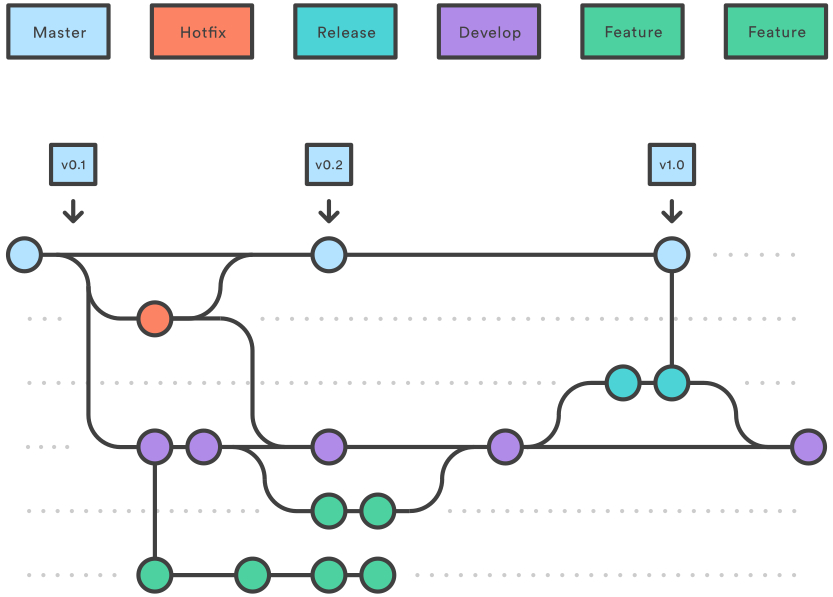
\includegraphics[width=\textwidth]{img/git-flow.jpg}

}

\caption{\label{fig-version-2}With Git}

}

\end{minipage}%

\end{figure}
\end{frame}

\section{Installation and configuration}




\begin{frame}[fragile]{Installing Git}
\protect\hypertarget{installing-git}{}
\underline{\textbf{Windows and Mac}}

Download and install Git from \url{https://git-scm.com/downloads}.

When done, open \texttt{Git\ Bash}

\underline{\textbf{Linux}}

Open a \texttt{Terminal} window and type:

\code{sudo\ apt\ install\ git\ git-lfs\ git-flow}
\end{frame}



\begin{frame}[fragile]{Git configuration: register who your are}

On \texttt{Git\ Bash} or in the \texttt{Terminal}:

Type
\code{git\ config\ -\/-global\ user.name\ "Firstname\ Lastname"}

Type \code{git\ config\ -\/-global\ user.email\ "myadresse@ird.fr"}

\textbf{N.B.} These two lines identify you in the history of a project.

Type \code{git\ config\ -\/-global\ -\/-list} to see the global git
configuration.
\end{frame}

\section{Getting started with Git in local}

% \begin{frame}[fragile]{Git architecture}
% \protect\hypertarget{git-architecture}{}
% \begin{figure}[H]

% {\centering \includegraphics[width=0.6\textwidth]{img/add_commit.png}

% }

% \end{figure}

% \begin{itemize}
% %\tightlist
% \item
%   \texttt{Repository}: a project Git
%   \item
%   \texttt{Stage} or \texttt{index}: the list of unvalidated changes 
%   \item
%   \texttt{add}: the command to add the file(s) to the list of tracked files
%   \item
%   \texttt{commit}: the command to validate a version
% \item
%   \texttt{Remote}: the remote version of the repository(ies) (GitHub,
%   GitlLab)
% \end{itemize}
% \end{frame}


\begin{frame}[fragile]{Git architecture}
\protect\hypertarget{git-architecture}{}
\begin{figure}[H]

{\centering 
\includegraphics[width=\textwidth]{mermaid/mermaid-figure-1.png}

}

\end{figure}

\begin{itemize}
%\tightlist
    \item
     \texttt{Workspace}: your working directory \(\rightarrow\) your
      computer
    \item
    \texttt{Local}: the local repository \(\rightarrow\) contains the
  history of your project
\item
  \texttt{Index} or \texttt{Stage}:  a buffer between \texttt{Workspace} and \texttt{Local}
  \(\rightarrow\) the list of files to be committed 
 \item
  \texttt{add}: the command to add the file(s) to the list of tracked files
  \item
  \texttt{commit}: the command to validate a version
\end{itemize}
\end{frame}

\begin{frame}[fragile]{Getting started}
\protect\hypertarget{getting-started}{}

Create a folder called \texttt{training-git} by typing
\code{mkdir\ training-git}

Move to the folder by typing \code{cd\ training-git}

Type \code{ls\ -alrt}

Type \code{git\ init}

Type again \code{ls\ -alrt}.

\textbf{N.B.} A \texttt{.git} folder has appeared. It contains the full history of
your project (\texttt{Local} repository)

Type \code{git\ status} and \code{git\ log}
\end{frame}

\begin{frame}[fragile]{First commit}
\protect\hypertarget{first-commit}{}

Create a \texttt{README.md} file. Type \code{git\ status}
\(\rightarrow\) \texttt{README.md} is now in \texttt{Workspace} but
not in \texttt{Local}

Type \code{git\ add\ README.md} and \code{git\ status}

\begin{figure}[H]

{\centering 
\includegraphics[width=0.4\textwidth]{mermaid/mermaid-figure-26.png}

}

\end{figure}

Type \code{git\ commit\ -m\ "First\ commit"} and type
\code{git\ log}

\begin{figure}[H]

{\centering 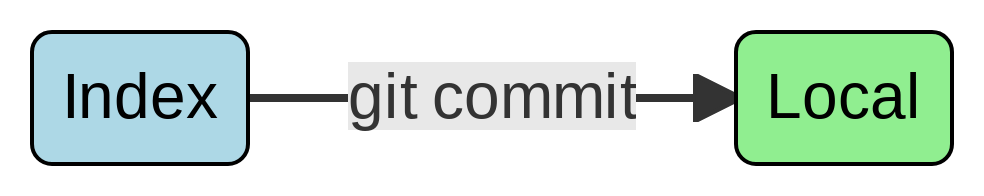
\includegraphics[width=0.4\textwidth]{mermaid/mermaid-figure-25.png}

}

\end{figure}

\begin{figure}[H]

{\centering 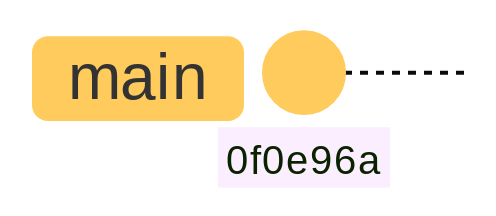
\includegraphics[width=0.2\textwidth]{mermaid/mermaid-figure-24.png}}

\end{figure}


\texttt{0f0e96a} is a short version of the identifier of the commit

\end{frame}

\begin{frame}[fragile]{Second commit}
\protect\hypertarget{second-commit}{}

Open the \texttt{README.md} file, add \texttt{\#\ Git\ training} and
save

Type \code{git\ status}

Type \code{git\ diff}

\begin{figure}[H]

{\centering 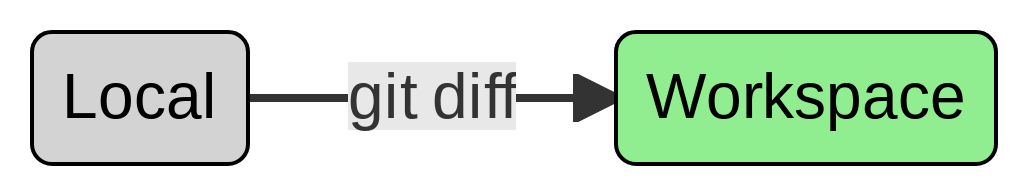
\includegraphics[width=0.5\textwidth]{mermaid/mermaid-figure-23.png}

}

\end{figure}

Type \code{git\ commit\ -m\ "Second\ commit"}

Type \code{git\ log}

\begin{figure}[H]

{\centering 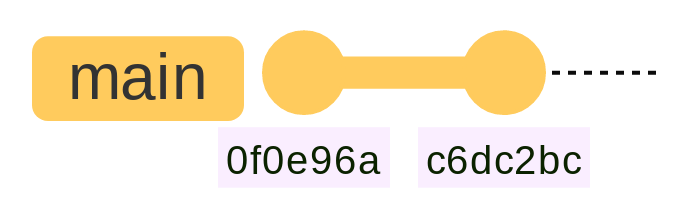
\includegraphics[width=0.3\textwidth]{mermaid/mermaid-figure-22.png}

}

\end{figure}
\end{frame}

\begin{frame}[fragile]{Creating tags}
\protect\hypertarget{creating-tags}{}

Open the \texttt{README.md} file and add
\texttt{\#\#\ Version\ v1.0.0}.

Type \code{git\ commit\ -m\ "Third\ commit"}

Type \code{git\ tag\ v1.0.0} and \code{git\ status}

\begin{figure}[H]

{\centering 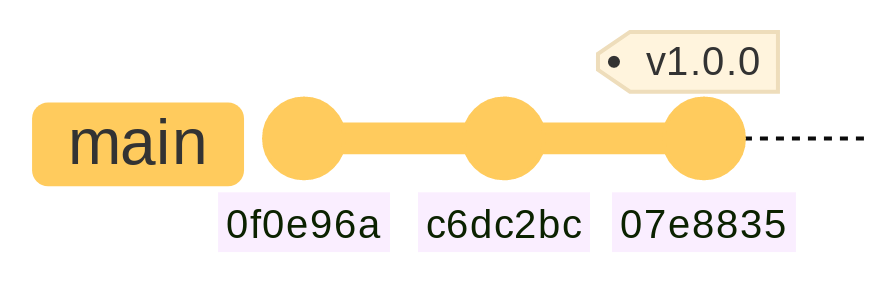
\includegraphics[width=0.4\textwidth]{mermaid/mermaid-figure-21.png}

}

\end{figure}

Type \code{git\ tag} to list all existing tags
\end{frame}

\begin{frame}[fragile]{Ignoring files}
\protect\hypertarget{ignoring-files}{}
It is possible to tell Git to ignore some files by using a
\href{https://git-scm.com/docs/gitignore}{.gitignore} file.

Create an empty \texttt{output.log} file and type \code{git\ status}

Create a \texttt{.gitignore} file and write \texttt{*.log}. Type again
\code{git\ status}

The \texttt{output.log} file no longer appears as \texttt{Untracked}

Type \code{git\ add\ .gitignore} and \code{git\ status}

Type \code{git\ commit\ -m\ "Fourth\ commit"}

\begin{figure}[H]

{\centering 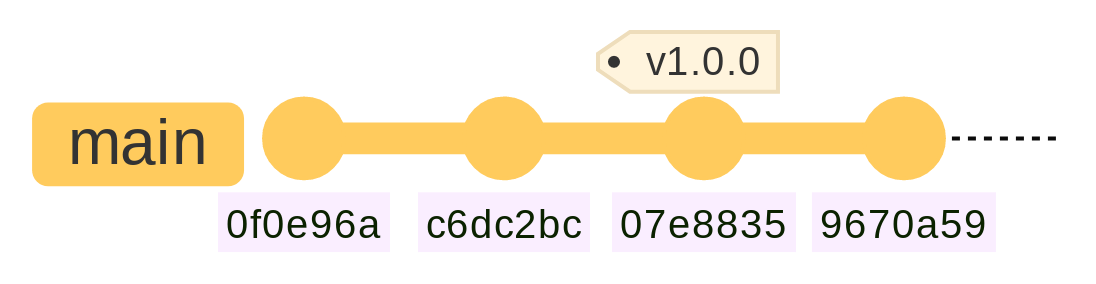
\includegraphics[width=0.5\textwidth]{mermaid/mermaid-figure-20.png}

}

\end{figure}

% \textbf{N.B.} To list the ignored files, type
% \code{git\ ls-files\ --others\ --ignored\ --exclude-from=.gitignore}

\end{frame}

\begin{frame}[fragile]{Moving in the history}
\protect\hypertarget{moving-in-the-history}{}

Type \code{git\ checkout\ v1.0.0} \(\rightarrow\) move to a tag

\begin{figure}[H]

{\centering 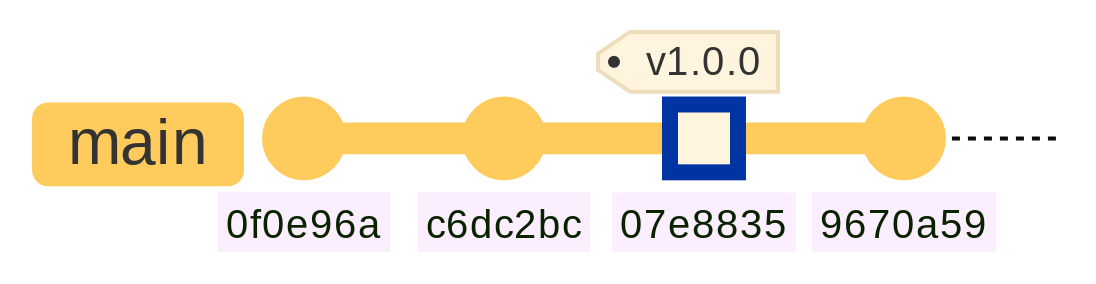
\includegraphics[width=0.4\textwidth]{mermaid/mermaid-figure-19.png}

}

\end{figure}

Type \code{git\ checkout\ 0f0e96a} \(\rightarrow\) move to the first
commit

\begin{figure}[H]

{\centering 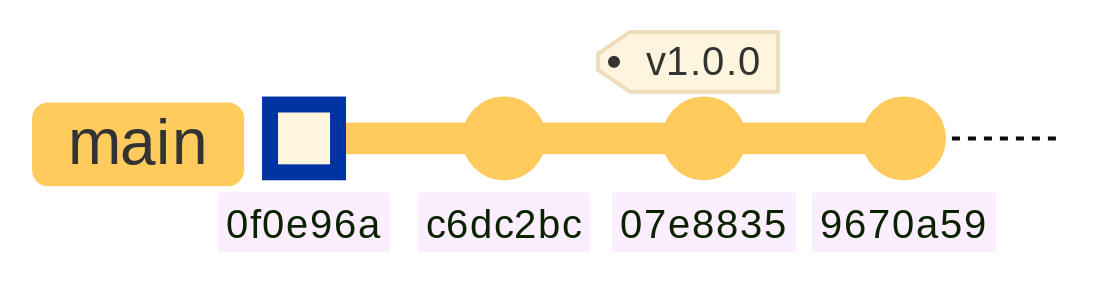
\includegraphics[width=0.4\textwidth]{mermaid/mermaid-figure-18.png}

}

\end{figure}

Type \code{git\ checkout\ main} \(\rightarrow\) move at the latest
commit

\begin{figure}[H]

{\centering 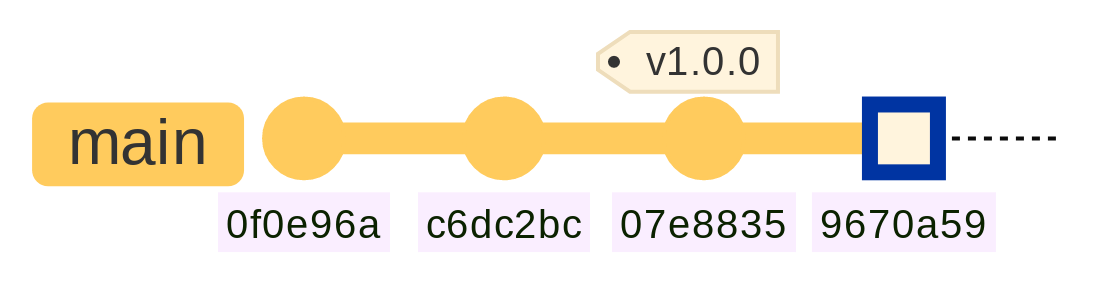
\includegraphics[width=0.4\textwidth]{mermaid/mermaid-figure-17.png}

}

\end{figure}

\textbf{N.B.} \texttt{HEAD} is a symbolic reference pointing to your location in history

\end{frame}

\begin{frame}[fragile]{Display differences}
\protect\hypertarget{display-differences}{}

Type \code{git\ diff\ 0f0e96a\ v1.0.0} \(\rightarrow\) compares a
commit and a tag.

\textbf{N.B.} Order matters when using \texttt{git\ diff}. Differences are shown with
the reference state considered to be the first argument.

\begin{figure}[H]

{\centering 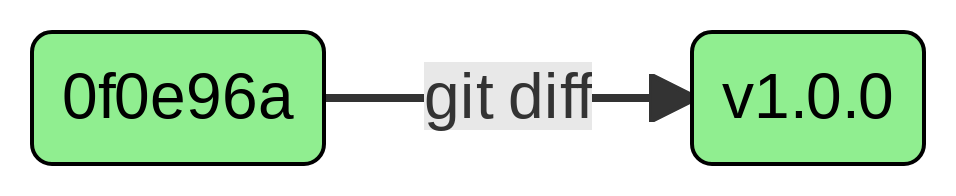
\includegraphics[width=0.4\textwidth]{mermaid/mermaid-figure-16.png}

}

\end{figure}

Type \code{git\ diff\ 0f0e96a\ c6dc2bc} \(\rightarrow\) compares two
commits.

Type \code{git\ diff\ 0f0e96a\ HEAD} \(\rightarrow\) compares where
you are in the history (\texttt{HEAD}) with a given commit.
\end{frame}

\section{Using Git with online server (GitHub)}



\begin{frame}[fragile]{Using remotes}
\protect\hypertarget{using-remotes}{}
In addition of saving the history, Git allows
to:

\begin{itemize}
%\tightlist
\item
  Save a project remotely

  \begin{itemize}
  %\tightlist
  \item
    Synchronization with different computers (laptop, HPCs)
  \end{itemize}
\item
  Share a project (codes, packages) with the community

  \begin{itemize}
  %\tightlist
  \item
    Reproducible science
  \end{itemize}
\end{itemize}

To do so, a \(4^{th}\) component in the Git architecture must be
considered: the \texttt{Remote} repository.


\begin{figure}[H]

{\centering 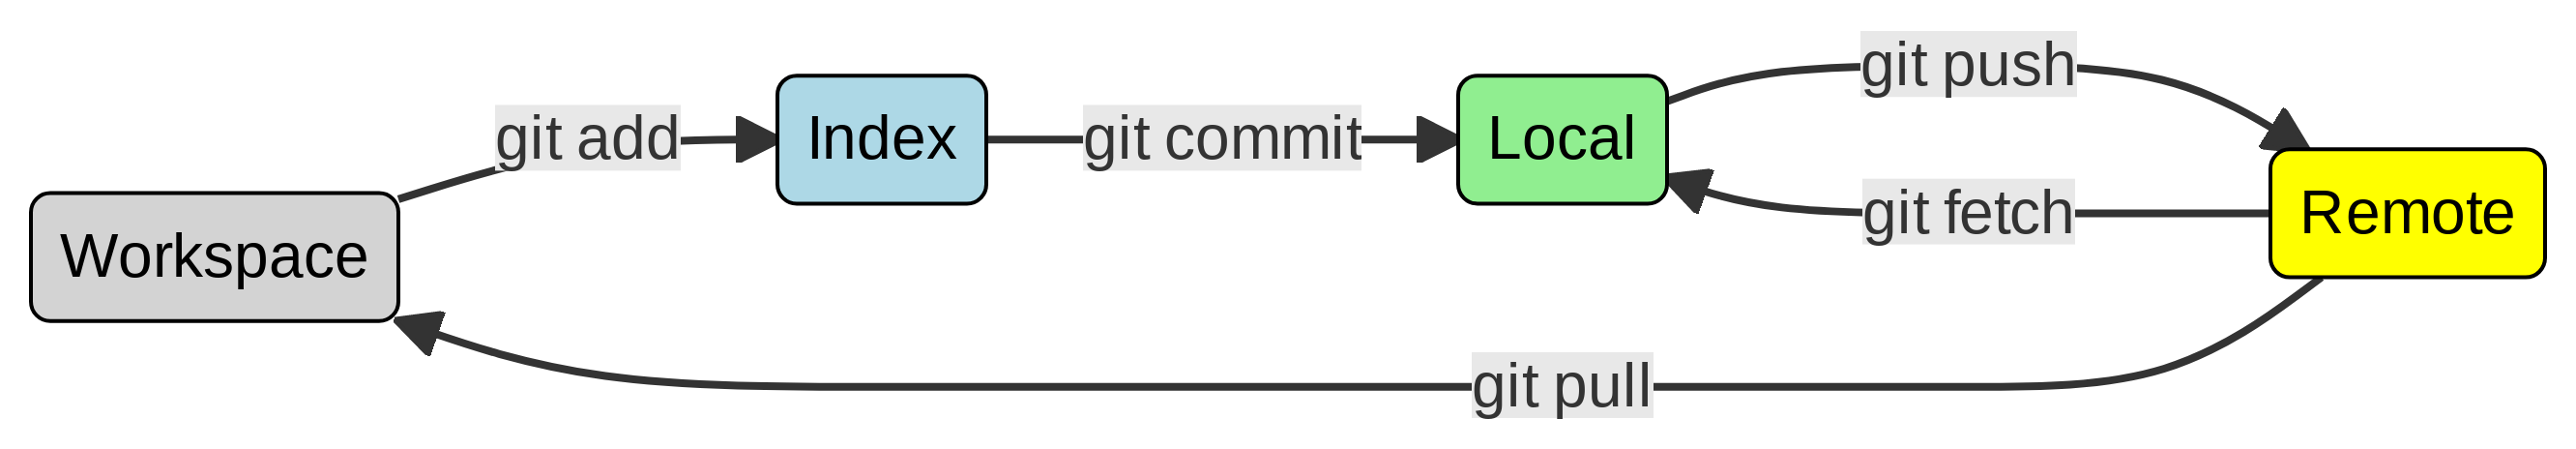
\includegraphics[width=\textwidth]{mermaid/mermaid-figure-15.png}

}

\end{figure}

It contains a \textbf{remote} version of the history of
your project
\end{frame}

\begin{frame}{Remote hosts}
\protect\hypertarget{remote-hosts}{}
There are several remote hosting possibilities:

\textbf{Commercial hosts}:

\begin{itemize}
%\tightlist
\item
  GitHub: \url{https://github.com/}
\item
  GitLab: \url{https://gitlab.com/}
\end{itemize}

\textbf{Institutional hosts}:

\begin{itemize}
%\tightlist
\item
  GitLab IRD: \url{https://forge.ird.fr/}
\item
  GitLab Ifremer \url{https://gitlab.ifremer.fr/}
\end{itemize}

In the following, we will use GitHub.



\textbf{N.B. }GitHub proposes extra-features for students, teachers and researchers.
Visit \url{https://education.github.com/benefits} for more information

\end{frame}

\begin{frame}[fragile]{Creation of a GitHub repository}
\protect\hypertarget{creation-of-a-github-repository}{}

On your GitHub page, click on \texttt{Repositories}

Click on the green \texttt{New} button

Set the name of your remote repository. Leave the other fields empty

Click on \texttt{Create\ repository}


\begin{figure}

{\centering 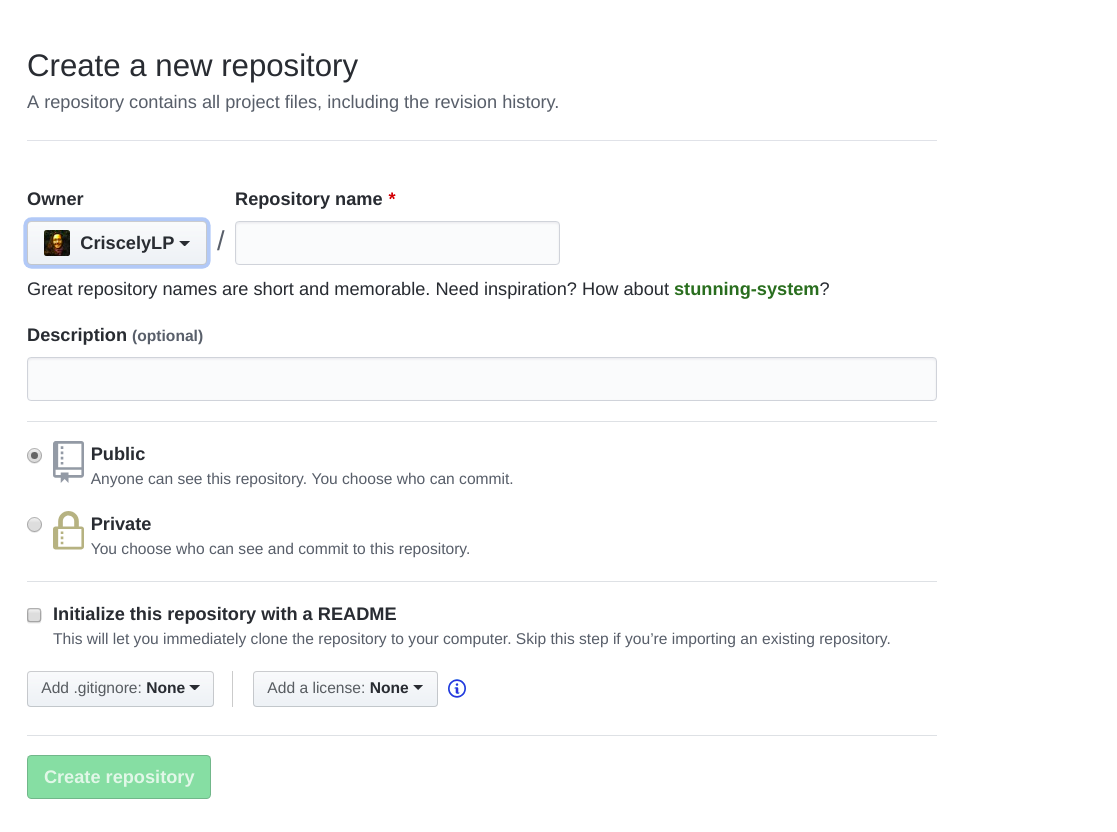
\includegraphics[width=0.7\textwidth]{img/github_makeRepo.png}

}

\end{figure}

\end{frame}

\begin{frame}[fragile]{Creation of a personal access token}

\begin{columns}
\begin{column}{0.6\textwidth}
   
To authenticate, you need to create an authentication token 
\href{https://docs.github.com/en/authentication/keeping-your-account-and-data-secure/creating-a-personal-access-token}{(see GitHub authentication for details)}

\vspace{0.5cm}
To do so, click on your profile photo and then on \texttt{Settings}:

\end{column}
\begin{column}{0.33\textwidth}  
    \begin{center}
     %%%%% this is a minipage, so \textwidth is already adjusted to the size of the column
     
\includegraphics[width=\textwidth]{img/github-settings.png}
     \end{center}
\end{column}
\end{columns}

\end{frame}

\begin{frame}[fragile]{Creation of a personal access token}
\protect\hypertarget{creation-of-a-personal-access-token-1}{}

In the left sidebar, click on \texttt{Developer\ settings}.

Under \texttt{Personal\ access\ tokens}, click
\texttt{Tokens\ (classic)}.

Select \texttt{Generate\ new\ token} and
\texttt{Generate\ new\ token\ (classic)}.

\begin{columns}
\begin{column}{0.3\textwidth}  
    \begin{center}
     %%%%% this is a minipage, so \textwidth is already adjusted to the size of the column
     
\includegraphics[width=\textwidth]{img/access-token-4.png}
     \end{center}
\end{column}
\begin{column}{0.3\textwidth}  
    \begin{center}
     %%%%% this is a minipage, so \textwidth is already adjusted to the size of the column
     
\includegraphics[width=\textwidth]{img/access-token-1.png}
     \end{center}
\end{column}
\begin{column}{0.3\textwidth}  
    \begin{center}

     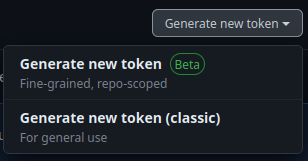
\includegraphics[width=\textwidth]{img/access-token-3.png}
     \end{center}
\end{column}
\end{columns}

\end{frame}

\begin{frame}[fragile]{Creation of a personal access token}
\protect\hypertarget{creation-of-a-personal-access-token-2}{}

Add some notes and \textbf{click on the \texttt{repo} box}, as shown
below:

\begin{figure}

{\centering 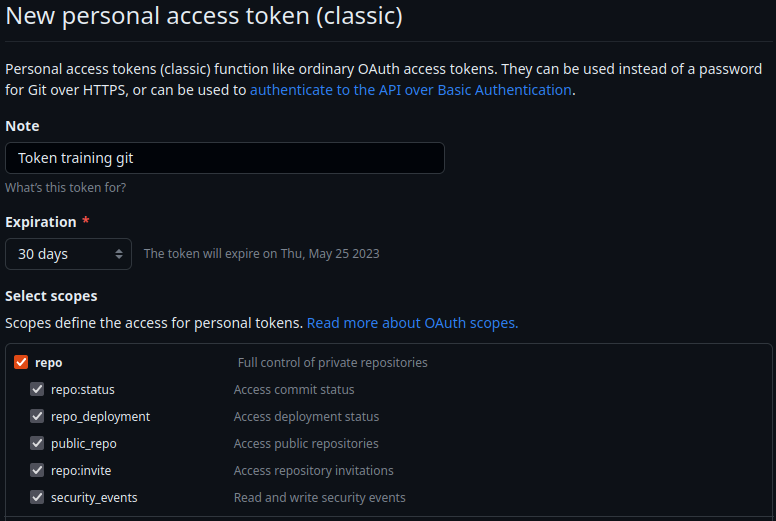
\includegraphics[width=0.6\textwidth]{img/access-token-2.png}

}

\end{figure}

Click on the \texttt{Generate\ token} box button.

\textbf{Copy and save in a \texttt{.txt} file the token: this is your
password!} 
\end{frame}

\begin{frame}[fragile]{Linking Git local and remote}
\protect\hypertarget{synchronization-to-the-remote}{}

In \texttt{Terminal} or \texttt{Git\ Bash}, copy and paste what is
shown on the GitHub page below the
\texttt{...or\ push\ an\ existing\ repository\ from\ the\ command\ line} instructions:

Type \code{
git\ remote\ add\ origin\ https://github.com/barriern/git-train.git
} by replacing \verb+barriern+ by your GitHub login

It connects your \verb+Local+ repository with a remote one, called
\emph{origin}

\begin{center}
 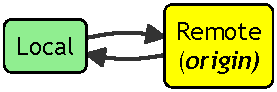
\includegraphics[width=0.4\textwidth]{mermaid/diagram-1-1.pdf}
\end{center}

Type \code{git\ remote\ -vv}

\end{frame}

\begin{frame}[fragile]{Linking Git local and remote}

Type \code{
git\ branch\ -M\ main
}

It renames the \verb+main+ or \verb+master+ branch to fit the remote branch name.

Type \code{git\ push\ -u\ origin\ main}

It connects the \emph{local} and \emph{remote} \verb+main+ branches (\verb+-u+ option) and sends the commits to the remote branch 

\begin{center}
 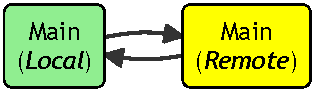
\includegraphics[width=0.4\textwidth]{mermaid/diagram-2-1.pdf}
\end{center}

\textbf{N.B}: \texttt{Username} is your GitHub login, \texttt{Password} is your token

Type \code{git\ branch\ -vv}

\end{frame}

\begin{frame}[fragile]{Linking Git local and remote}

Have a look at your repository on GitHub. \textbf{Tags are missing!}

Type \code{git\ push\ --tags} and refresh the GitHub page.
 
\begin{center}
    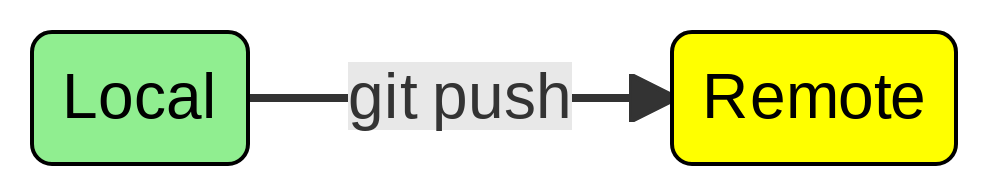
\includegraphics[width=0.4\textwidth]{mermaid/mermaid-figure-14.png}
\end{center}

\textbf{N.B}: No need to specify the \verb+-u origin main+ option since the two branches are already connected.

Navigate on the GitHub page to see what has been done

\end{frame}

\begin{frame}[fragile]{Linking Git local and remote}
\protect\hypertarget{synchronization-from-the-remote}{}
In GitHub, click on the \texttt{README.md} file and then on the edit
button

Add a \texttt{Update\ from\ Github} line and click on
\texttt{Commit\ changes}

\begin{figure}

\begin{minipage}[b]{0.45\linewidth}

{\centering 

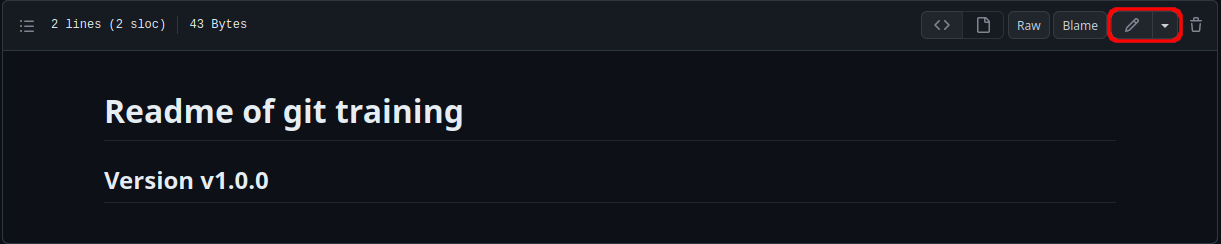
\includegraphics[width=\textwidth]{img/readme-edit.png}

}

\end{minipage}%
%
\begin{minipage}[b]{0.45\linewidth}

{\centering 

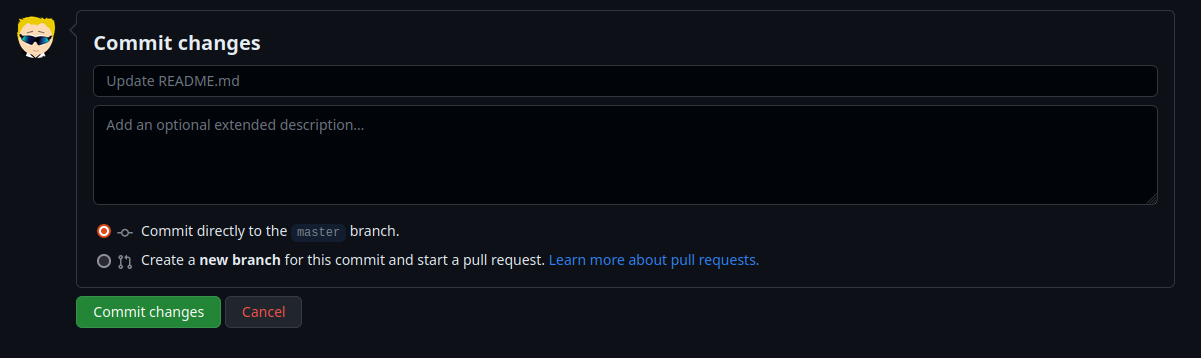
\includegraphics[width=\textwidth]{img/readme-edit-2.png}

}

\end{minipage}%

\end{figure}

Loot at the \verb+README.md+ file on your computer. The \texttt{Remote} changes are not visible yet in
\texttt{Workspace}

In \texttt{Git\ Bash} or \texttt{Terminal}, type \code{git\ pull}

\begin{center}
\begin{figure}[H]
     
\includegraphics[width=0.4\textwidth]{mermaid/mermaid-figure-13.png}
     \end{figure}
\end{center}

Look again at the \verb+README.md+ file on your computer


\end{frame}

\begin{frame}{Synchronization: conflicts}
\protect\hypertarget{synchronization-conflicts}{}

On GitHub, add \texttt{x\ =\ 1} at the end of the \texttt{README.md}
file. \textbf{Do not pull!}

On your computer, edit the \texttt{README.md} and add
\texttt{x\ =\ 2}.

Type \code{git\ commit\ -m\ "Fifth\ commit"}

Type \code{git\ push}. An error occurs because changes in
\texttt{Remote} are not in \texttt{Local}.

Type \code{git\ pull} and \code{git\ status}.

It says that a conflict has occurred on the \texttt{README.md} file.
This is due to diverging history.

\begin{figure}[H]

{\centering 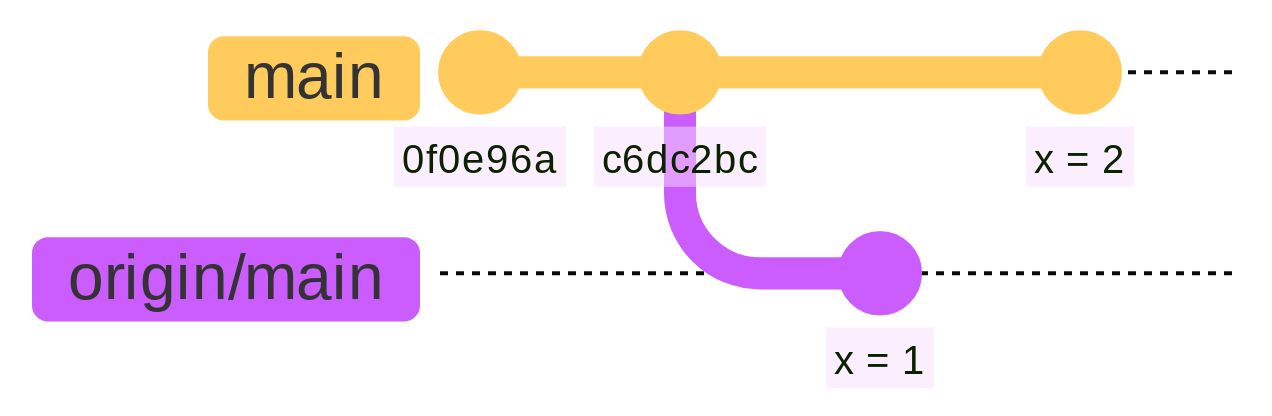
\includegraphics[width=0.6\textwidth]{mermaid/mermaid-figure-12.png}

}

\end{figure}
\end{frame}

\begin{frame}[fragile]{Synchronization: conflicts}
\protect\hypertarget{synchronization-conflicts-1}{}

Open the \texttt{README.md} file. You should see:

\begin{verbatim}
<<<<<<< HEAD
x = 2
=======
x = 1
>>>>>>> 70a4c105e377db282c0769606960f0afcccdd071
\end{verbatim}
\textbf{N.B.} These are conflicts markers. \texttt{Git} doesn't know whether to chose
\texttt{x\ =\ 1} or \texttt{x\ =\ 2}. \textbf{This is your job!!}

Open the file, replace the 3 lines above by \texttt{x\ =\ 3}. Commit and push
the changes

\begin{figure}[H]

{\centering 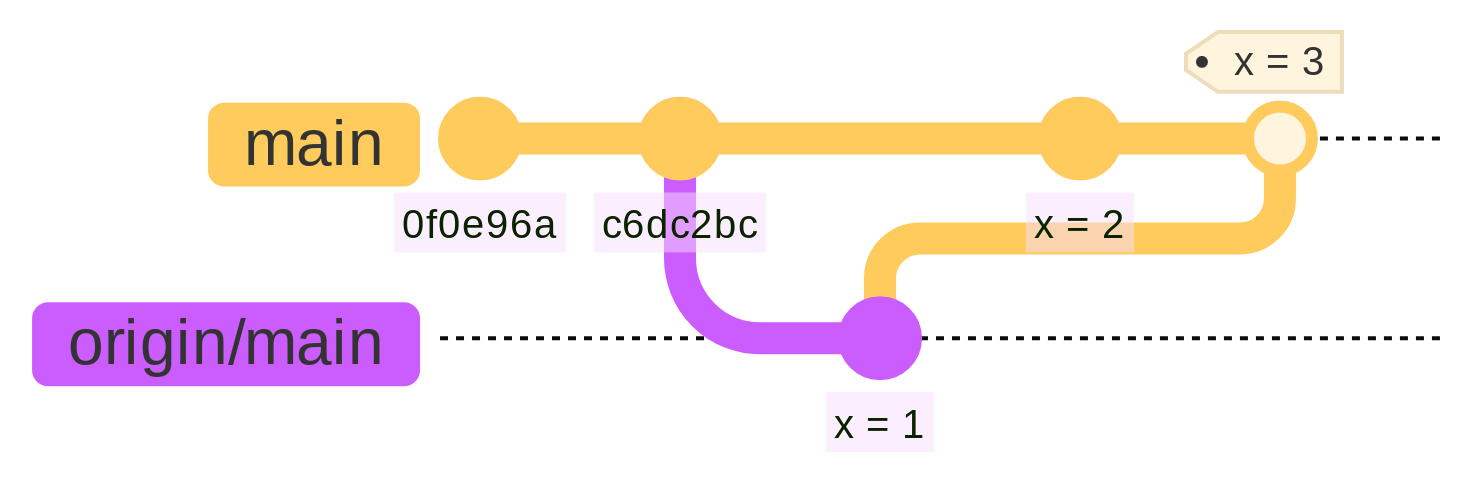
\includegraphics[width=0.6\textwidth]{mermaid/mermaid-figure-11.png}

}

\end{figure}
\end{frame}

\begin{frame}[fragile]{Cloning an existing repository}
\protect\hypertarget{cloning-an-existing-repository}{}

In \texttt{Terminal} or \texttt{Git\ Bash}, type \code{cd\ ..}

Now type \code{git\ clone\ https://github.com/umr-marbec/git-training}

\begin{figure}[H]

{\centering 
\includegraphics[width=0.4\textwidth]{mermaid/mermaid-figure-10.png}

}

\end{figure}

Type \code{git\ log} to see the full history.

To update the project, type \code{git\ pull}

\textbf{N.B. Do not clone or initialize a Git repository in another Git
repository!}

\end{frame}

\begin{frame}[fragile]{Conclusion: good practice}
\protect\hypertarget{conclusion-good-practice}{}
\begin{itemize}
%\tightlist
\item
  Before starting editing a project, do a \code{git\ pull}
\item
  Commit very often using \code{git\ commit} extensively
\item
  Push often as well using \code{git\ push}
\item
  Use \code{git\ status} extensively to know what you have done
\end{itemize}

\begin{figure}

{\centering 
\includegraphics[width=0.5\textwidth]{img/funny.jpg}

}

\end{figure}
\end{frame}

\section{Git clients (IDE)}

\begin{frame}{Git clients}
\protect\hypertarget{git-clients}{}
Git Clients are softwares that facilitate the use of Git (see
\href{https://git-scm.com/downloads/guis}{Git Guis} for a list).

Besides, most code editors include Git functionalities
\end{frame}

\begin{frame}{Git clients}
\protect\hypertarget{git-clients-1}{}
\begin{figure}

{\centering 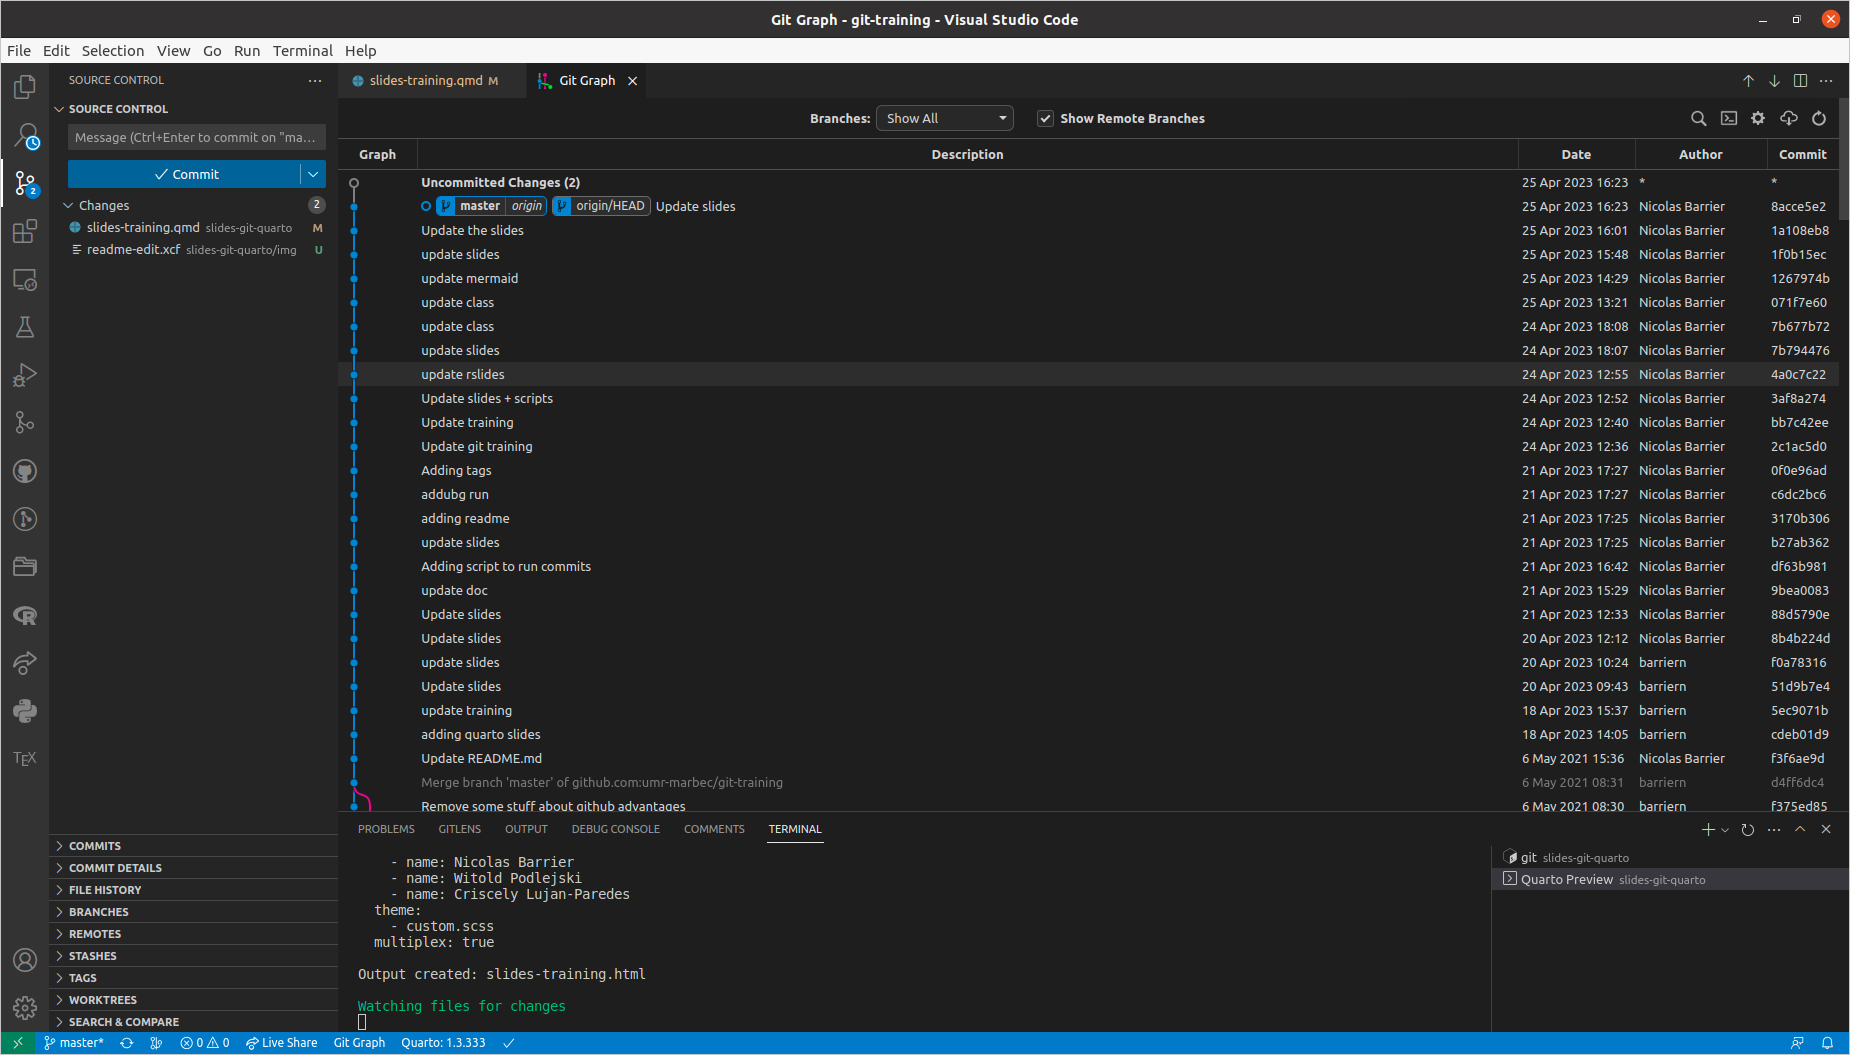
\includegraphics[width=\textwidth]{img/vscode.png}

}

\caption{\label{fig-vscode}VSCode}

\end{figure}
\end{frame}

\begin{frame}{Git clients}
\protect\hypertarget{git-clients-2}{}
\begin{figure}

{\centering 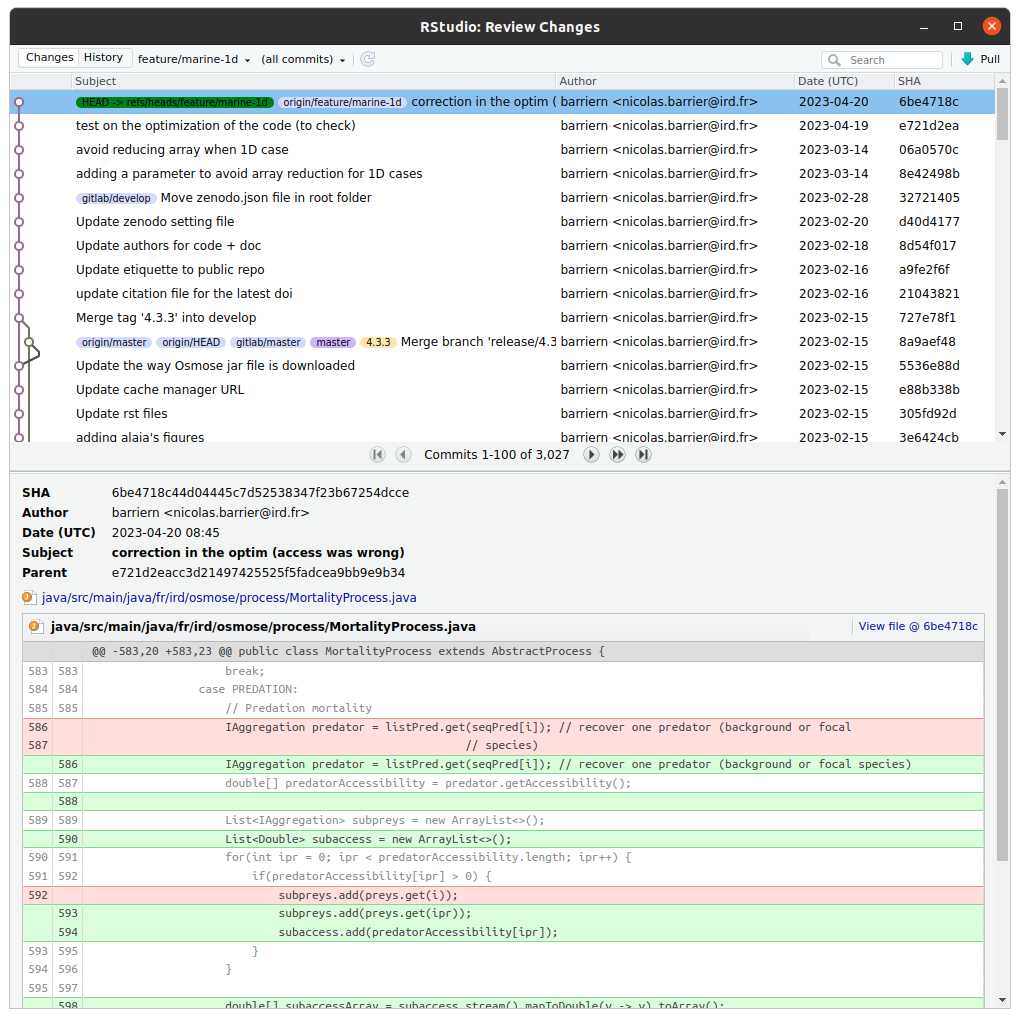
\includegraphics[width=0.7\textwidth]{img/rstudio.png}

}

\caption{\label{fig-rstudio}RStudio}

\end{figure}
\end{frame}

\begin{frame}{Git clients}
\protect\hypertarget{git-clients-3}{}
\begin{figure}

{\centering 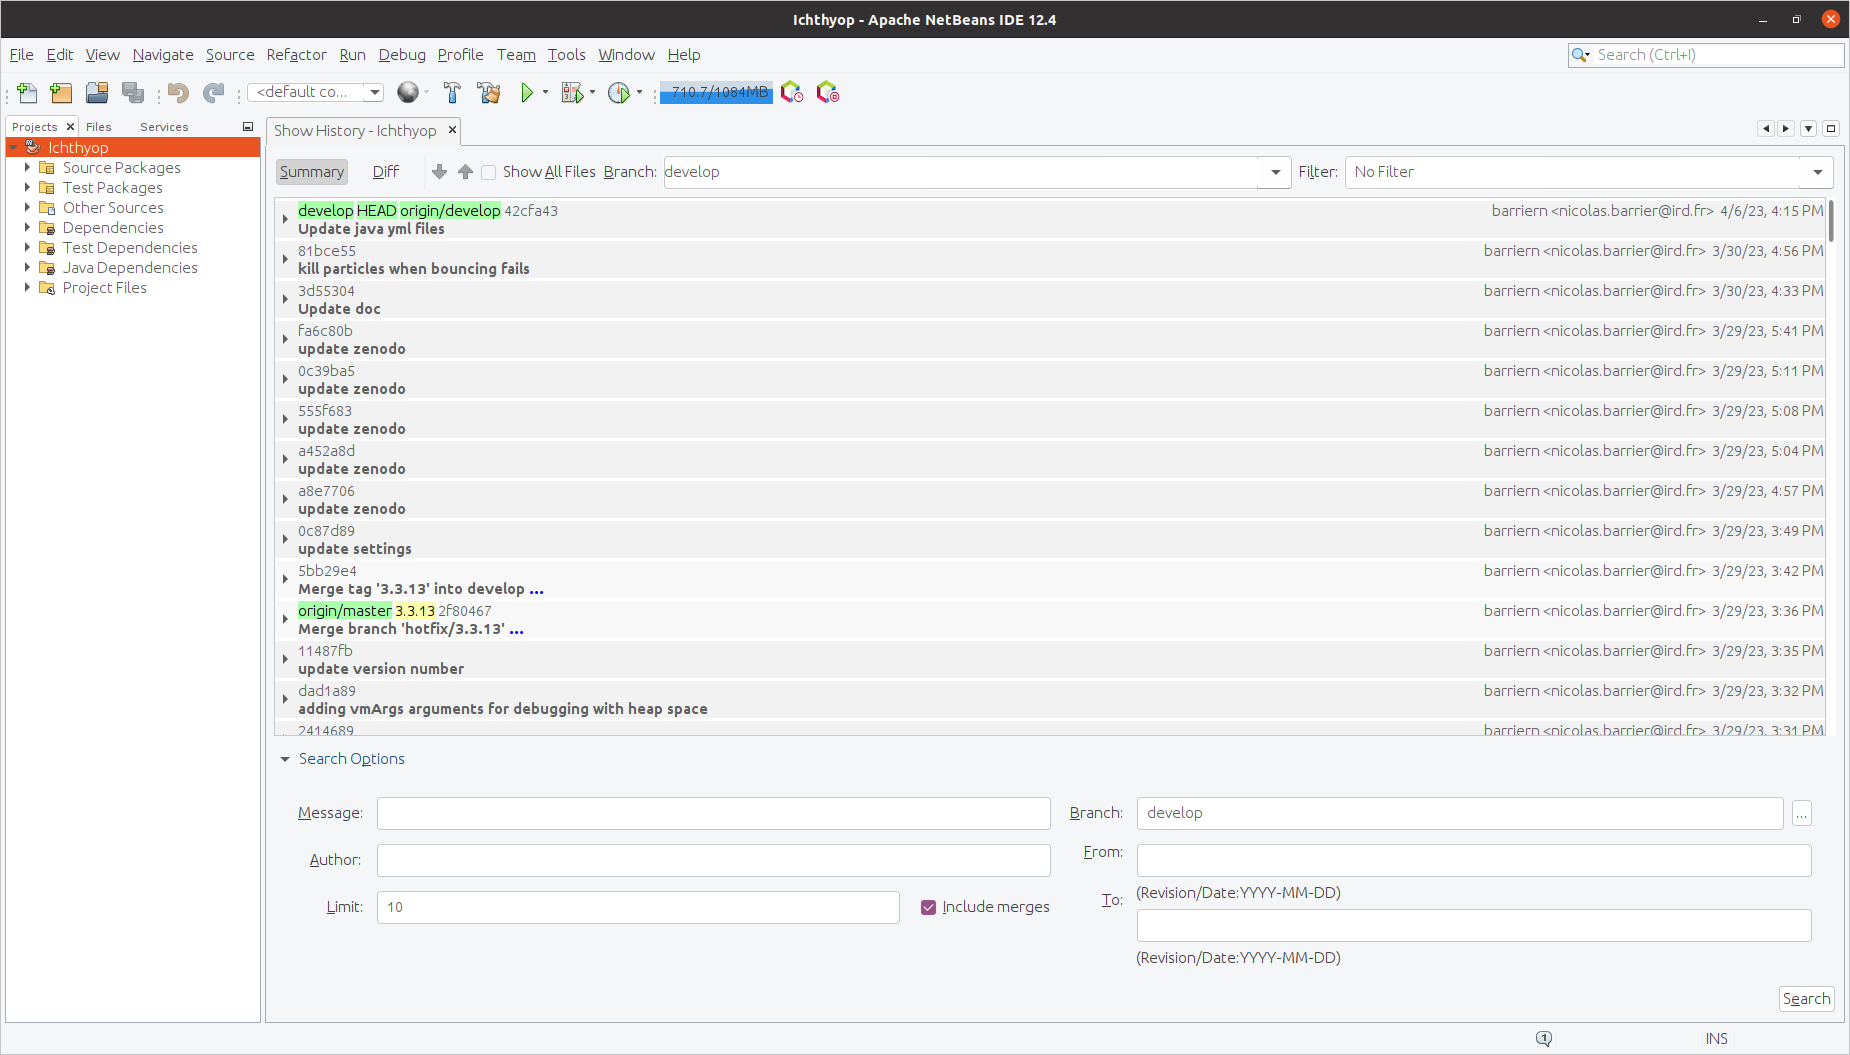
\includegraphics[width=0.9\textwidth]{img/netbeans.png}

}

\caption{\label{fig-netbeans}Netbeans}

\end{figure}
\end{frame}

\begin{frame}{Going further\ldots{}}
\protect\hypertarget{going-further}{}
For those who want, extra slides are available on:

\begin{itemize}
%\tightlist
\item
  Working with branches, i.e.~derivates of a project
\item
  Git with \href{https://git-lfs.github.com/}{Large File Storage}
  extension.
\end{itemize}

\begin{figure}[H]

{\centering 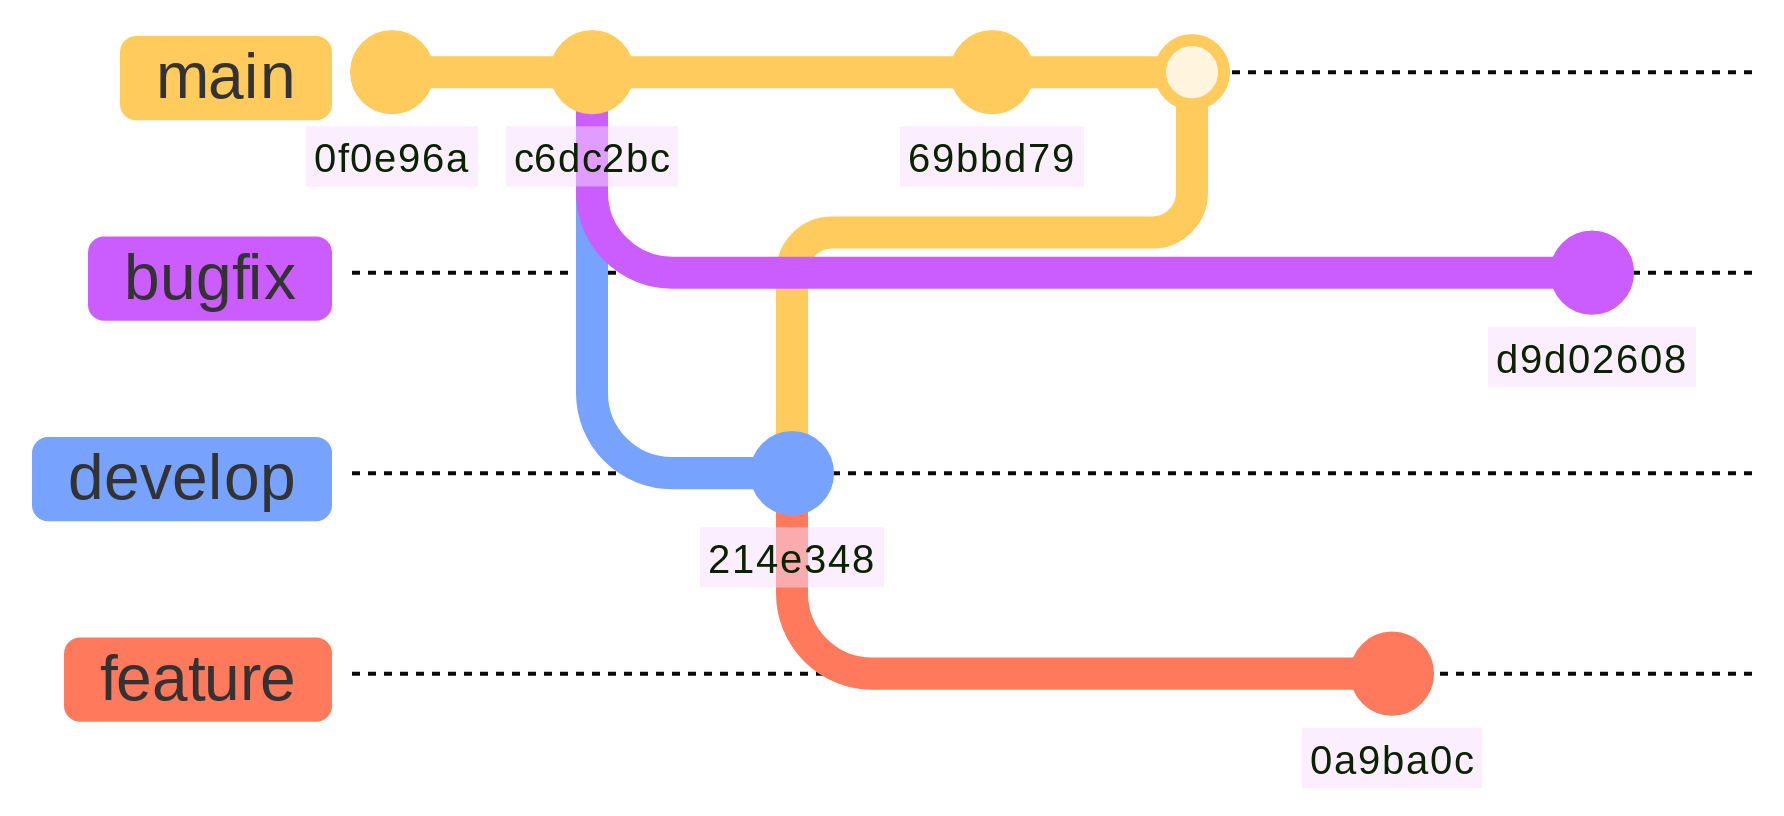
\includegraphics[width=0.8\textwidth]{mermaid/mermaid-figure-9.png}

}

\end{figure}
\end{frame}

\section{Use of multiples projects derivates (branches)}

\begin{frame}[fragile]{Creating aliases}
\protect\hypertarget{creating-aliases}{}
Before working with branches, we will create some Git aliases (i.e.~shortcuts):

Type
\code{git\ config\ -\/-global\ alias.tree\ log\ -\/-all\ -\/-decorate\ -\/-oneline\ -\/-graph}

Type \code{git\ config\ --global\ alias.br\ branch\ -vv}

Type \code{git\ config\ -\/-global\ alias.re\ remove\ -vv}

\end{frame}


\begin{frame}[fragile]{Creating branches}
\protect\hypertarget{creating-branches}{}

Type \code{git\ checkout\ -b\ develop}

Type \code{git\ status}, \code{git\ br} and \code{git\ tree}

Open the \texttt{README.md} file, add some text and save.

Type \code{git\ add\ README.md}

Type \code{git\ commit\ -m\ "Update readme.md"}

Type \code{git\ br} and \code{git\ tree}


\begin{figure}[H]

{\centering 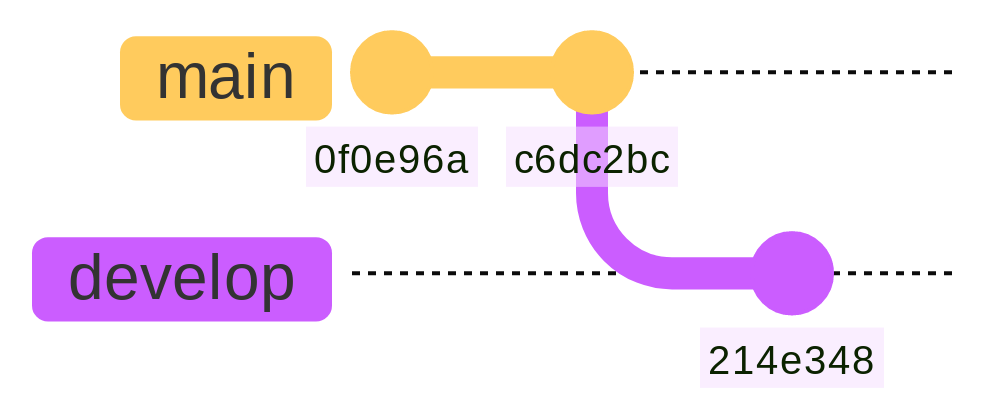
\includegraphics[width=0.6\textwidth]{mermaid/mermaid-figure-8.png}

}

\end{figure}
\end{frame}

\begin{frame}[fragile]{Switching branch}
\protect\hypertarget{switching-branch}{}

Type \code{git\ checkout\ main} (or \code{git\ checkout\ master})

Type \code{git\ br}

Create a \texttt{LICENCE} file and add some text in it

Type \code{git\ add\ LICENCE}

Type \code{git\ commit\ -m\ "Adding\ LICENCE file"}

Type \code{git\ tree}


\begin{figure}[H]

{\centering 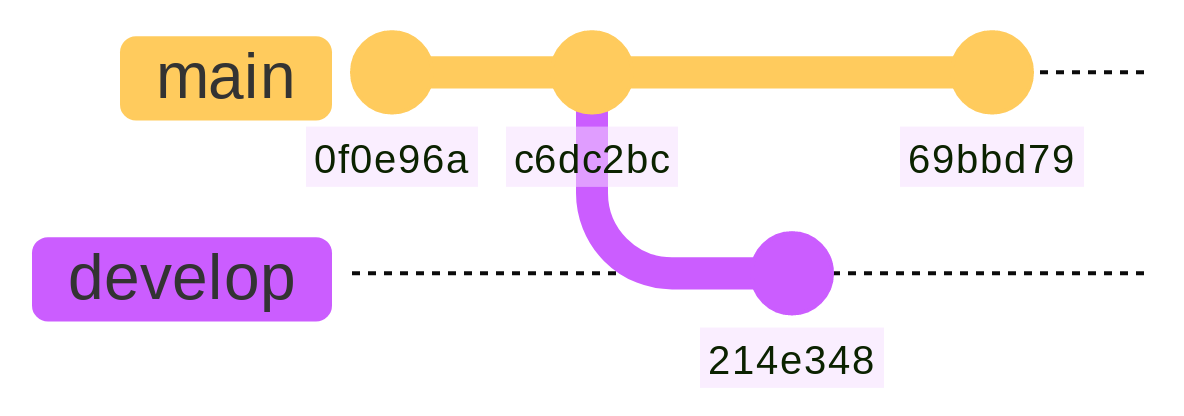
\includegraphics[width=0.6\textwidth]{mermaid/mermaid-figure-7.png}

}

\end{figure}
\end{frame}

\begin{frame}[fragile]{Merging branches}
\protect\hypertarget{merging-branches}{}

On the \texttt{main} branch, type
\code{git\ merge\ develop\ -m\ "merge-develop"}

Type \code{git\ log} and \code{git\ tree}

\begin{figure}[H]

{\centering 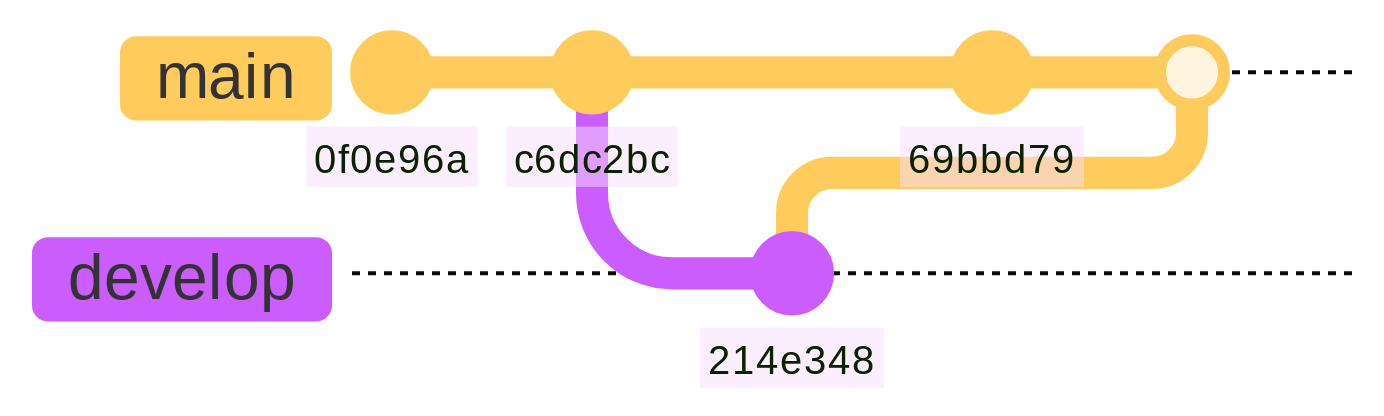
\includegraphics[width=0.7\textwidth]{mermaid/mermaid-figure-6.png}

}

\end{figure}

The \texttt{merge} command takes the commits (\verb+214e348+) from the argument branch
(\texttt{develop}) and includes them into the current branch (here
\texttt{main}).


\textbf{N.B. }During the merging process, another commit is created, which contains the changes of both \verb+214e348+ and \verb+69bbd79+ commits

\end{frame}

\begin{frame}[fragile]{Creating branch from another branch}
\protect\hypertarget{creating-branch-from-another-branch}{}

Type \code{git\ checkout\ -b\ feature\ develop}

Create a \texttt{script.R} file

Type \code{git\ add\ script.R}

Type \code{git\ commit\ -m\ "Fourth\ commit"}


\begin{figure}[H]

{\centering 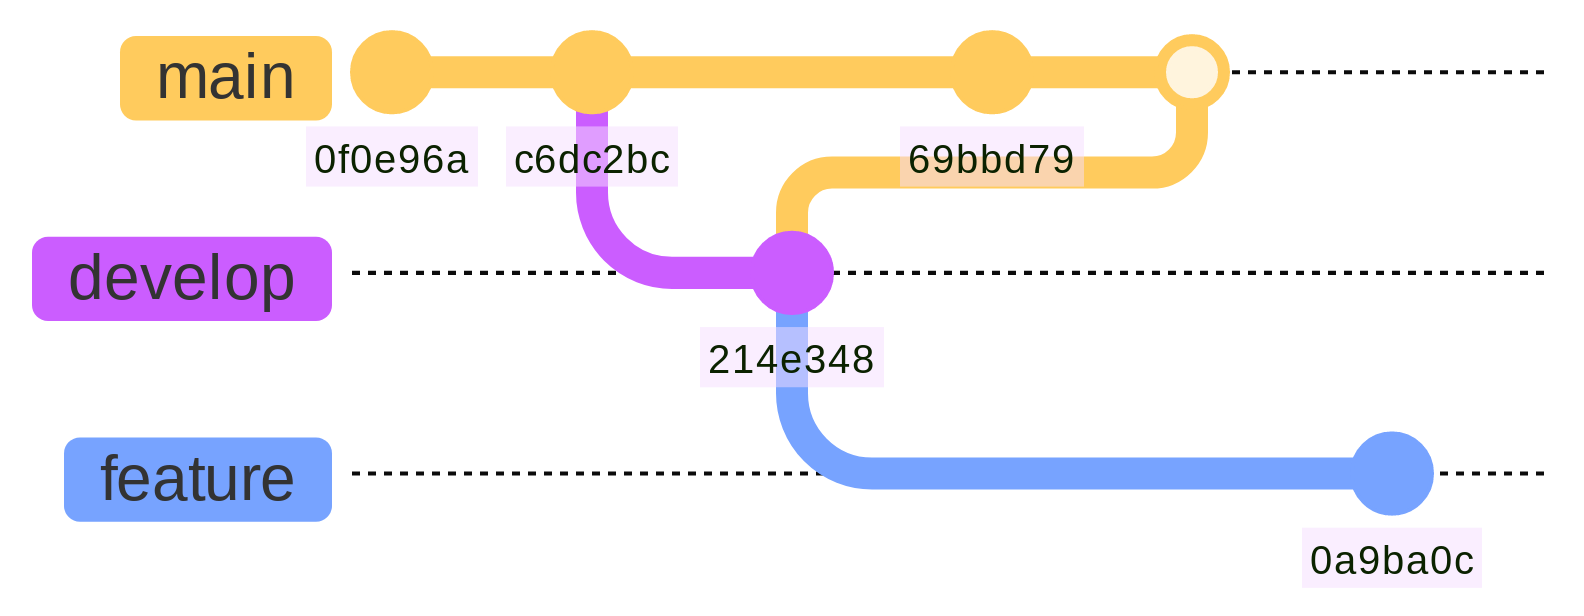
\includegraphics[width=0.8\textwidth]{mermaid/mermaid-figure-5.png}

}

\end{figure}
\end{frame}

\begin{frame}[fragile]{Creating branch from a commit}
\protect\hypertarget{creating-branch-from-a-commit}{}

Type \code{git\ checkout\ -b\ feat-com\ c6dc2bc} replacing
\texttt{c6dc2bc} by an actual commit ID.

Create a \texttt{script.py} file

Type \code{git\ add\ script.py} and
\code{git\ commit\ -m\ "Sixth\ commit"}


\begin{figure}[H]

{\centering 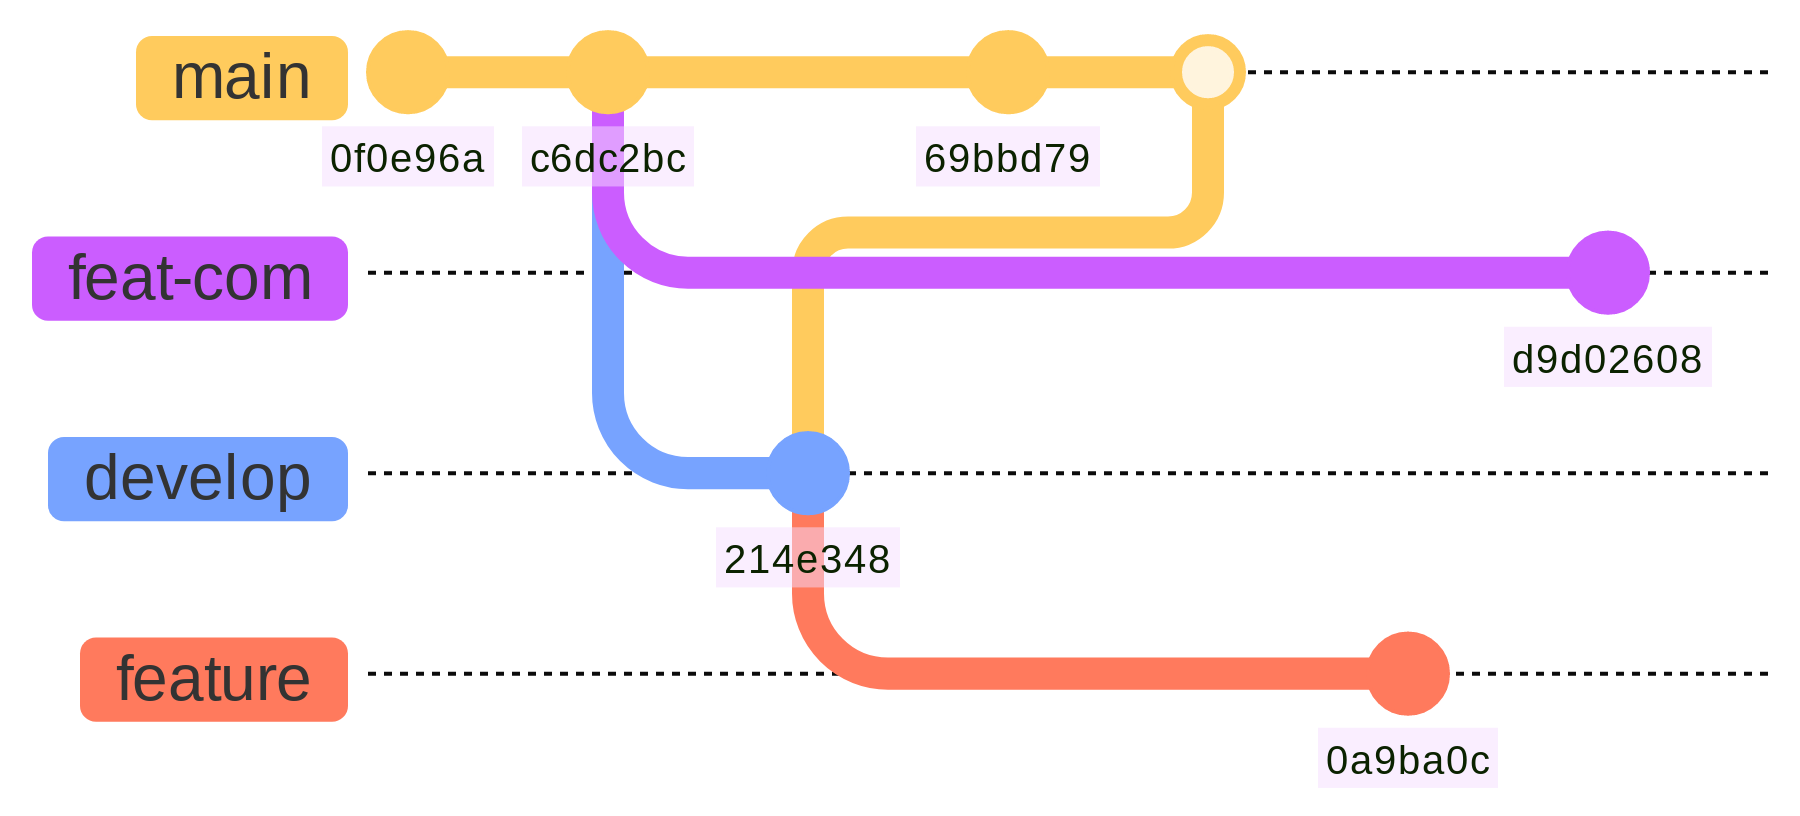
\includegraphics[width=0.6\textwidth]{mermaid/mermaid-figure-4.png}

}

\end{figure}
\end{frame}

\begin{frame}[fragile]{Differences between branches}
\protect\hypertarget{differences-between-branches}{}

Type \code{git\ diff\ main\ develop}

\note{You will see the text that has been added to the LICENCE file
(69bbd79 commit)}


\textbf{N.B. }Order matters: it shows what has been added to \texttt{main} branch
compared to the \texttt{develop} branch

\begin{figure}[H]

{\centering 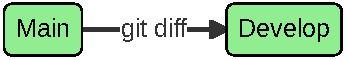
\includegraphics[width=0.6\textwidth]{mermaid/diagrams-1.pdf}

}

\end{figure}

Type \code{git\ diff\ main\ feat-com}

\end{frame}

\begin{frame}[fragile]{Deleting a branch}
\protect\hypertarget{deleting-a-branch}{}

Type \code{git\ checkout\ main}

Type \code{git\ branch\ -d\ develop}

Type \code{git\ br}

Type \code{git\ branch\ -d\ feature}


An error occurs! The suppression of \texttt{feature} implies the loss
of the \texttt{0a9ba0c} commit. To force the suppression, use
\texttt{-D} instead of \texttt{-d}.

Type \code{git\ branch\ -D\ feature}

\textbf{N.B. }The suppression of \texttt{develop} was ok because the content of commit
\texttt{214e348} is included in the merge.

\end{frame}

\begin{frame}[fragile]{Branches in remote}

Type \code{git\ checkout feat-com}

To push a branch on the remote repository:

Type \code{git\ push -u origin feat-com}

\begin{figure}[H]

{\centering 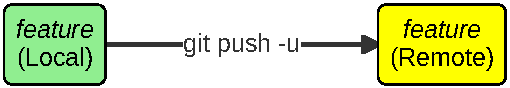
\includegraphics[width=0.6\textwidth]{mermaid/diagrams-2.pdf}

}

\end{figure}

To list the remote branches, type \code{git branch -a}

To track a remote branch, type \code{git checkout remote-branch}, with
\verb+remote-branch+ the name of the branch

\begin{figure}[H]

{\centering 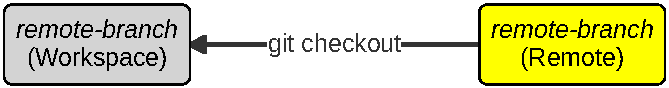
\includegraphics[width=0.7\textwidth]{mermaid/diagrams-3.pdf}

}

\end{figure}

\end{frame}

% \begin{frame}[fragile]{Reverting a commit}
% \protect\hypertarget{reverting-a-commit}{}

% Type \code{git\ revert\ c6dc2bc} (replace \texttt{c6dc2bc} by your
% commit id)

% \begin{figure}[H]

% {\centering 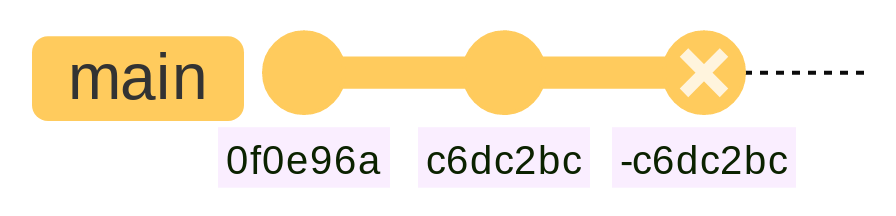
\includegraphics[width=0.35\textwidth]{mermaid/mermaid-figure-2.png}

% }

% \end{figure}
% \end{frame}

\section{Working with large files}

\begin{frame}[fragile]{Large file storage}
\protect\hypertarget{large-file-storage}{}
To version (reasonably) large files (\verb+.nc+, \verb+.csv+)
\(\rightarrow\) \href{https://git-lfs.github.com/}{LFS extension}


\textbf{N.B. }Make sure that the remote host is compatible with LFS (GitHub is
compatible)

Type \code{git\ lfs\ install} to activate the extension

Create a \texttt{data.csv} file and add \texttt{Year,Size,Species}

Type \code{git\ lfs\ track\ "*.csv"}


A \texttt{.gitattributes} file has appeared, which list all the file
extensions managed by Git LFS.
\end{frame}

\begin{frame}[fragile]{Large file storage}
\protect\hypertarget{large-file-storage-1}{}

Type \code{git\ add\ .gitattributes\ data.csv}

Type \code{git\ commit\ -m\ "Using\ LFS"}

Type \code{git\ push}

On GitHub, click on your file \texttt{data.csv} file.

\end{frame}

\begin{frame}{Sources}
\protect\hypertarget{sources}{}
\begin{itemize}
%\tightlist
\item
  Plateau bioinformatique, Montpellier: Formation Git(Lab) (05/04/2018)
\item
  UMR AMAP (Atelier MAIA P3M), Montpellier: Introduction à GIT
  (04/04/2019)
\item{\textbf{For the bold:} the full Git documentation (506 pages!): \url{https://git-scm.com/book/en/v2}}
\end{itemize}

\end{frame}

\end{document}

